%!TEX root = /Users/louis/Documents/PhD/Deliverables/Thesis/thesis.tex

\subsection{Exemplar User-Driven Co-Evolution}
The analysis presented in Chapter~\ref{Analysis} led to the discovery of user-driven co-evolution, in which model migration is not executable and is instead performed by hand. Chapter~\ref{Analysis} highlighted two challenges faced when user-driven co-evolution techniques are applied. Firstly, model storage representations have not been optimised for use by humans, and hence user-driven co-evolution can be error-prone and time consuming. Secondly, when a multi-pass parser is used to load models (as is the case with EMF), user-driven co-evolution is an iterative process, because not all conformance errors are reported at once. These challenges led to the derivation of the following research requirement: \emph{This thesis must demonstrate a user-driven co-evolution process that enables the editing of non-conformant models without directly manipulating the underlying storage representation and provides a conformance report for the original model and evolved metamodel.}

Chapter~\ref{Implementation} presented two tools that seek to fulfil the above research requirement. The first, metamodel-independent syntax, facilitates the conformance checking of a model against any metamodel. Conformance checking can be manual (invoked by the user) or automatic (via integration of the metamodel-independent syntax with a framework for monitoring workspace changes, as described in Section~\ref{subsec:automatic_checking}). The second tool, an implementation of the textual modelling notation HUTN, allows models to be managed in a format that is reputedly easier for humans to use than the canonical model storage format, XMI \cite{hutn}.

This section demonstrates a user-driven co-evolution process which uses the conformance reporting and textual modelling notation described in this thesis. To this end, an example of co-evolution, based on changes observed in the process-oriented project described in Chapter~\ref{Analysis}, is used throughout the remainder of this section. The example is used to show the way in which user-driven co-evolution might be achieved with and without the conformance reporting and textual modelling notation described in Chapter~\ref{Implementation}.

\subsubsection{Co-Evolution Example}
The co-evolution example used throughout this section is based on changes observed in the process-oriented project, which was described in Chapter~\ref{Analysis}. The metamodel considered was developed in joint work with Adam Sampson, a research associate at the University of Kent. The work involved building a prototypical tool for editing graphical models of process-oriented programs. EuGENia \cite{kolovos09eugenia} was used to automatically generate a graphical editor from the process-oriented metamodel. The metamodel was developed iteratively in the following manner:

\begin{enumerate}
	\item Draw by hand a desired graphical model for a simple process-oriented program.
	\item Change the metamodel to capture any new or revised domain concepts.
	\item Regenerate the graphical editor from the metamodel.
	\item Use the editor to draw the desired graphical model.
	\item Check that the current (and all previous) graphical models are satisfactory representations of their hand-drawn counterparts.
\end{enumerate}

After step 5, work continued by returning to step 2 if the computerised graphical model was not a satisfactory representation of the hand-drawn model created in step 1. Otherwise, work continued by returning to step 1. The metamodel was completed after 6 iterations. Each iteration produced a new pair of hand-drawn and computerised graphical models. To prevent regressions, step 5 checked the current pair and all previous pairs of models.

Here, one iteration of the process-oriented metamodel is considered, which led to the metamodel changes shown in Figure~\ref{fig:po_mms}. In Figure~\ref{fig:original_po_mm}, a \texttt{Pr\-og\-r\-am} is composed of \texttt{Channel}s and \texttt{Co\-nn\-ec\-ti\-onPo\-in\-t}s. A \texttt{Ch\-an\-n\-el} reads from and writes to exactly one \texttt{Co\-nn\-ec\-ti\-o\-nPo\-i\-nt}. Further analysis of the domain revealed that \texttt{Co\-nn\-ec\-ti\-o\-nPo\-i\-nt}s may only be used for reading or for writing, and never both. To capture this constraint, \texttt{Co\-nn\-ec\-ti\-o\-nPo\-i\-nt} was made abstract, and two subtypes, \texttt{Re\-ad\-i\-ngCo\-nn\-ec\-ti\-o\-nPo\-i\-nt} and \texttt{Wr\-i\-ti\-ngCo\-nn\-ec\-ti\-o\-nPo\-i\-nt}, were introduced. The reader and writer references of \texttt{Ch\-an\-n\-el} then referred to the new subtypes, as shown in Figure~\ref{fig:evolved_po_mm}.

\begin{figure}[htbp]
	\centering
	\subfigure[Original metamodel.]
	{
	    \label{fig:original_po_mm}
	    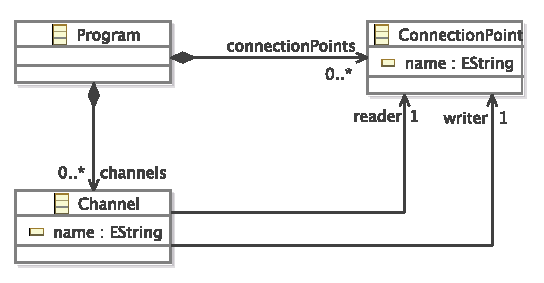
\includegraphics[width=6cm]{6.Evaluation/images/po_before.pdf}
	}
	\subfigure[Evolved metamodel.]
	{
	    \label{fig:evolved_po_mm}
	    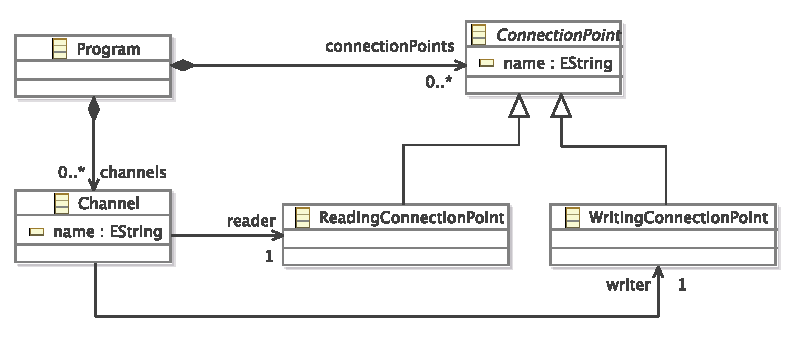
\includegraphics[width=8cm]{6.Evaluation/images/po_after.pdf}
	}
	\caption{Process-oriented metamodel evolution.}
\label{fig:po_mms}
\end{figure}

In general, changes made during step 2 of the process described above could cause models previously created during step 5 to become non-conformant. For the process-oriented metamodel, a user-driven co-evolution process was preferred to a developer-driven co-evolution process because they were only a small number of models (at most 5) to be migrated.

When the process-oriented metamodel was developed, no tools were available for performing user-driven co-evolution. Migration was performed by editing the storage representation of the models, which was error-prone and time-consuming. This process is now described, and is then compared to a user-driven co-evolution process that uses the conformance checking tool and the textual modelling notation described in Chapter~\ref{Implementation}.

\subsubsection{Existing Process}
The process-oriented metamodel was developed before the conformance reporting tool and textual modelling notation described in Chapter~\ref{Implementation} were implemented. As such, model migration involved attempting to load existing, potentially non-conformant models with EMF, noting any conformance errors and changing the corresponding XMI to make the model conform to the evolved metamodel.

For the metamodel changes shown in Figure~\ref{fig:po_mms}, conformance errors were reported for all of the existing models. Initially, two types of messages were received for non-conformant models. For every instance of \texttt{Co\-nn\-ec\-ti\-o\-nPo\-i\-nt}, the following message was produced: ``Class `ConnectionPoint' is not found or is abstract.'' For every instance of \texttt{Ch\-an\-n\-el} that referenced a \texttt{Co\-nn\-ec\-ti\-o\-nPo\-i\-nt}, the following message was produced: ``Unresolved reference `\texttt{<ID>}' '' where \texttt{<ID>} was the identifier of the referenced \texttt{Co\-nn\-ec\-ti\-o\-nPo\-i\-nt}.

To fix both types of error, the XMI of each model was changed such that each instance of \texttt{Co\-nn\-ec\-ti\-onPo\-in\-t} was replaced by an instance of \texttt{Re\-ad\-i\-ngCo\-nn\-ec\-ti\-o\-nPo\-i\-nt} or \texttt{Wr\-i\-ti\-ngCo\-nn\-ec\-ti\-o\-nPo\-i\-nt}. This involved adding an extra attribute, \texttt{xsi:type}, to each \texttt{Co\-nn\-ec\-ti\-onPo\-in\-t}, a rather technical process, which is discussed further below.

In a small number of cases, the wrong subtype of \texttt{Co\-nn\-ec\-ti\-onPo\-in\-t} was selected, probably because XMI identifies elements using randomly generated strings rather than a domain-specific naming scheme. In one model, two connection points named \texttt{a\_reader} and \texttt{a\_writer} had the very similar XMI IDs \texttt{\_MeFREC8sEd69s-McmXQlqQ} and \texttt{\_M7EvEC8sEd69s-McmXQlqQ}, respectively. Because of this, the two connection points were assigned the wrong types when the XMI was changed by hand.

Conformance errors are reported only when a model is loaded by EMF (and hence, in this case, only when the graphical editor is used to open a model). In other words, when the XMI of a model is changed by hand, conformance is not checked when the model is saved to disk. When the wrong subtype of  \texttt{Co\-nn\-ec\-ti\-onPo\-in\-t} was selected, the following message was produced when the model was opened with the graphical editor: ``Value `po.im\-pl.Re\-ad\-i\-ngCo\-nn\-ec\-ti\-onPo\-i\-nt@7f\-de\-16\-84 (name: a\_writer)' is not legal.'' After changing \texttt{xsi:type} attributes to instantiate the correct subtypes of \texttt{Co\-nn\-ec\-ti\-onPo\-in\-t}, all of the models could be opened without error by the graphical editor.


\subsubsection{Proposed Process}
A user-driven co-evolution process using the conformance reporting tool and the textual modelling notation, HUTN, presented in Chapter~\ref{Implementation} is now described. The new process involves invoking the conformance reporting tool to determine which models have conformance problems, generating HUTN for each non-conformant model, and fixing the conformance problems in the HUTN.

For the metamodel changes shown in Figure~\ref{fig:po_mms}, the conformance reporting tool reports three types of error message when invoked on non-conformant models\footnote{As described in Section~\ref{subsec:automatic_checking}, the conformance reporting tool can be invoked manually, via a context menu, or automatically as a result of integration with Concordance.}. For every instance of \texttt{Co\-nn\-ec\-ti\-o\-nPo\-i\-nt}, the following message is produced: ``Cannot instantiate the abstract class: ConnectionPoint.'' For every instance of \texttt{Ch\-an\-n\-el}, the following two error messages are produced: ``Expected ReadingConnectionPoint for: reader'' and ``Expected WritingConnectionPoint for: writer.''

To fix the errors, a HUTN representation of each non-conformant model is generated by invoking the ``Generate HUTN'' context menu item. Figure~\ref{fig:po_hutn} shows the HUTN generated for one of the non-conformant process-oriented models. Fixing the conformance problems involves changing the HUTN source by hand (and then regenerating the XMI using the ``Generate Model'' context menu item). For the model shown in Figure~\ref{fig:po_hutn}, fixing the conformance problems involved changing the type of \texttt{a\_reader} to \texttt{Re\-ad\-i\-ngCo\-nn\-ec\-ti\-o\-nPo\-i\-nt} and the type of \texttt{a\_writer} to \texttt{Wr\-i\-ti\-ngCo\-nn\-ec\-ti\-o\-nPo\-i\-nt}. Whenever the user saves the HUTN document, both syntax and conformance are checked by the background incremental compiler. Any problems are reported while the model is migrated.

\begin{figure}[htbp]
  \centering
  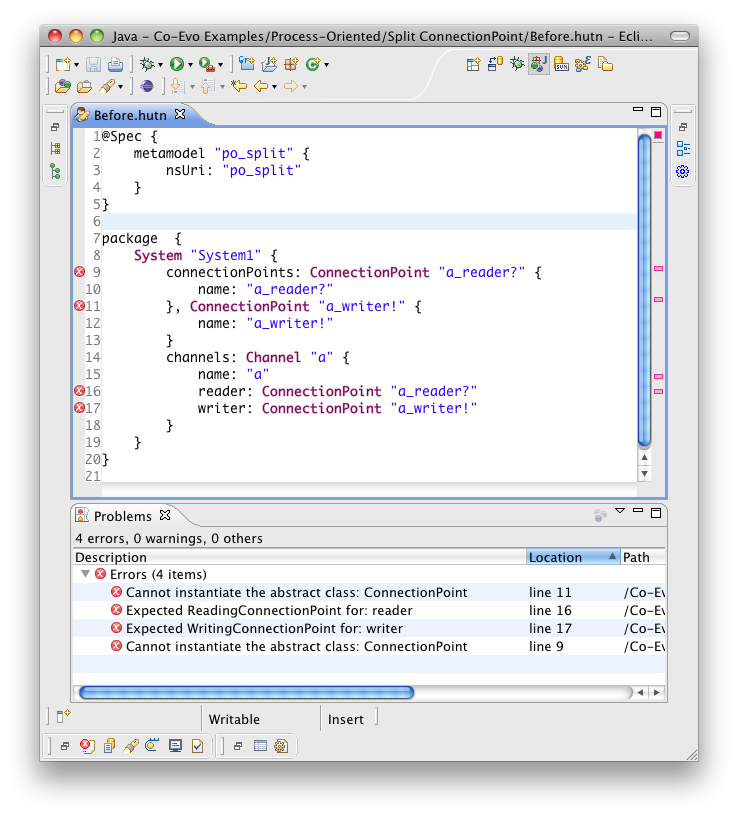
\includegraphics[width=13.5cm]{6.Evaluation/images/po_hutn.png}
  \caption{HUTN for a non-conformant process-oriented model.}
  \label{fig:po_hutn}
\end{figure}

\subsubsection{Summary}
This section has demonstrated existing and new user-driven co-evolution processes using an example of metamodel changes. Comparison of the two highlights several benefits of the new process, which used tools described in Chapter~\ref{Implementation}.

Firstly, the conformance reporting tool presented in Section~\ref{sec:mmi_syntax} can report more types of conformance problem at once than the model loading mechanism of EMF because the former uses a multi-pass parser, while the latter uses a single-pass parser. For the metamodel changes shown in Figure~\ref{fig:evolved_po_mm}, both the conformance reporting tool and the EMF loading mechanism reported that the evolved metamodel did not permit instantiation of the abstract class \texttt{Co\-nn\-ec\-ti\-o\-nPo\-i\-nt}. Another type of conformance problem -- the type of \texttt{Ch\-an\-n\-el\#re\-ad\-er} (\texttt{Ch\-an\-n\-el\#wr\-it\-er}) must be a \texttt{Re\-ad\-i\-ngCo\-nn\-ec\-ti\-o\-nPo\-i\-nt} (\texttt{Wr\-i\-ti\-ngCo\-nn\-ec\-ti\-o\-nPo\-i\-nt}) -- was reported by the conformance reporting tool when it was first invoked and reported by the loading mechanism of EMF only when it was invoked after the first category of conformance problem was fixed.

Secondly, the implementation of HUTN described in Section~\ref{sec:notation} uses a background incremental compiler that checks both the syntax and conformance of the HUTN source code. On the other hand, EMF checks conformance only when a model is loaded (by the graphical model editor, in this case). Saving XMI to disk does not cause EMF to check its conformance.

Thirdly, migration involved changing the types of some model elements. In XMI, when the type of a model element can be inferred from the context in which it is instantiated, type information is omitted. This reduces the size of the model on disk, but can be problematic for model migration. For example, in the original process-oriented metamodel (Figure~\ref{fig:original_po_mm}) any model element contained in the \texttt{Pr\-og\-r\-am\#co\-nn\-ec\-ti\-onPo\-in\-ts} reference must be an instance of \texttt{Co\-nn\-ec\-ti\-onPo\-in\-t}, and type information can be omitted from the XMI. When the process-oriented metamodel evolved to allow \texttt{Re\-ad\-i\-ngCo\-nn\-ec\-ti\-o\-nPo\-i\-nt} and \texttt{Wr\-i\-ti\-ngCo\-nn\-ec\-ti\-o\-nPo\-i\-nt}s to be contained in the \texttt{Pr\-og\-r\-am\#co\-nn\-ec\-ti\-onPo\-in\-ts}, type information must be added. To add type information to XMI, the person performing migration must know the correct syntax, for example: \texttt{xsi:type="po.Re\-ad\-i\-ngCo\-nn\-ec\-ti\-onPo\-i\-nt"}. By contrast, the type of every model element is declared explicitly in HUTN. As such, every HUTN document contains examples of how type information should be specified. Hence, changing the type of a model element in HUTN is arguably more straightforward than in XMI.

Finally, migration involved understanding which \texttt{Ch\-an\-n\-el}s referenced which \texttt{Co\-nn\-ec\-ti\-onPo\-in\-t}s.  By default, EMF uses universally unique identifiers (UUIDs) such as \texttt{\_M7EvEC8sEd69s-McmXQlqQ} -- or URI fragments (document-specific relative paths) such as \texttt{\\@co\-nn\-ec\-ti\-onPo\-in\-ts.0} -- to identify model elements. By contrast, the implementation of HUTN described in Chapter~\ref{Implementation}, uses the value of a model element's name feature (where one is defined) to identify model elements. For example, in \ref{fig:po_hutn} the \texttt{Ch\-an\-n\-el} on line 14 refers to \texttt{Co\-nn\-ec\-ti\-onPo\-in\-t}s by name (lines 16 and 17). Hence, referencing and dereferencing model elements in HUTN is arguably more straightforward than in XMI.

Further research is required to more rigorously assess the differences between the two user-driven co-evolution processes discussed in this section. In particular, the textual modelling notation used in the proposed process, HUTN, purports to be human-usable \cite{hutn}, but no usability studies have compared HUTN with other model representations, such as XMI. The implementation of tools for performing user-driven co-evolution, described in Chapter~\ref{Implementation}, enable further comparisons, but a thorough investigation of their usability is beyond the scope of this thesis.

This section has used two of the tools described in Chapter~\ref{Implementation} to demonstrate a user-driven co-evolution process that provides a conformance report and allows the editing of non-conformant models in a textual modelling notation. The benefits of the proposed process have been highlighted by comparison to an existing user-driven co-evolution process using a co-evolution example, taken from a project that used user-driven co-evolution.